\documentclass{beamer}
\usepackage{amsfonts,amsmath,oldgerm}
\usepackage{fancyvrb}
\usepackage{pgfplots}
\pgfplotsset{width=1cm, compat=1.9, every non boxed x axis/.append style={x axis line style=-},
     every non boxed y axis/.append style={y axis line style=-}}
\usetheme{sintef}
\definecolor{LightGray}{gray}{0.9}


% \setbeameroption{show notes on second screen}


\newcommand{\testcolor}[1]{\colorbox{#1}{\textcolor{#1}{test}}~\texttt{#1}}

\usefonttheme[onlymath]{serif}

\titlebackground*{assets/background}

\newcommand{\hrefcol}[2]{\textcolor{cyan}{\href{#1}{#2}}}

\title{Sviluppo di un sistema per rilevare spostamenti in auto tramite il Bluetooth degli smartphone}
\course{Laurea in Informatica}
\author{Antonio Pietro Romito}
\IDnumber{1932500}
\date{Anno Accademico 2023/2024}

\begin{document}
\maketitle
\note[itemize]{
\item Presenterò il lavoro svolto durante il mio tirocinio presso il Gamification Lab del Dipartimento di Informatica
\item sviluppo di un software in grado di rilevare automaticamente gli spostamenti in auto attraverso l'utilizzo del Bluetooth degli smartphone
\item Questo sistema è stato implementato all'interno dell'applicazione Android del progetto Generocity
}

\begin{sidepic}{assets/gc_home.png}{GeneroCity}
    \framesubtitle{Un'applicazione di smartparking}
    \begin{itemize}
        \item Applicazione Android e iOS sviluppata dal GamificationLab
        \item Facilita la ricerca dei parcheggi in un'area urbana
        \item Non richiede l'attenzione dell'utente
        \item Utilizzo sicuro alla guida
    \end{itemize}
    
\end{sidepic}
\note[itemize]{
\item applicazione di smart parking
\item attualmente in sviluppo per Android e iOS dal Gamification Lab
\item scopo: facilitare la ricerca dei parcheggi all’interno di un’area urbana
\item consente di farlo in maniera sicura senza causare distrazioni durante la guida
\item dato che non richiede l'attenzione dei suoi utenti
}

\section{Interazioni implicite}
\note[itemize]{
\item Ciò è possibile grazie all'impiego di interazioni implicite.
}

\begin{frame}{Cos'è un'interazione implicita}
\begin{columns}
    \begin{column}{0.4\textwidth}
        Interazione uomo macchina:
        \begin{itemize}
            \item non richiede comandi espliciti
            \item utilizza il contesto come input per l'elaborazione
        \end{itemize}
    \end{column}
    \begin{column}{0.6\textwidth}
        \begin{figure}
            \centering
            \includegraphics[width=\linewidth]{assets/context_aware.png}
        \end{figure}
    \end{column}
\end{columns}
\end{frame}
\note[itemize]{
\item Con questa espressione si intende un tipo di interazione uomo-macchina che non richiede dei comandi espliciti da parte dell’utente
\item piuttosto utilizza il contesto in cui quest’ultimo agisce come input per l’elaborazione
\item approccio fondamentale per garantire la sicurezza degli utenti durante la guida
}

\begin{frame}{I sensori}
\vspace{0.5cm}
\begin{columns}
    \begin{column}{0.95\textwidth}
        In GeneroCity un sensore è un modulo software che, analizzando il contesto in cui agisce l’utente in uno specifico istante, determina l’azione compiuta da quest’ultimo.
    \end{column}
\end{columns}
\vspace{0.5cm}

\begin{columns}
    \begin{column}{0.15\linewidth}
    \end{column}
    \begin{column}{0.15\linewidth}
        \begin{figure}
            \centering
            \includegraphics[width=0.7\linewidth]{assets/ic_gps.png}
        \end{figure}
    \end{column}
    \begin{column}{0.15\linewidth}
        \begin{figure}
            \centering
            \includegraphics[width=0.8\linewidth]{assets/ic_battery.png}
        \end{figure}
    \end{column}
    \begin{column}{0.15\linewidth}
        \begin{figure}
            \centering
            \includegraphics[width=0.9\linewidth]{assets/ic_bluetooth.png}
        \end{figure}
    \end{column}
    \begin{column}{0.15\linewidth}
        \begin{figure}
            \centering
            \includegraphics[width=0.8\linewidth]{assets/ic_cell.png}
        \end{figure}
    \end{column}
    \begin{column}{0.15\linewidth}
        \begin{figure}
            \centering
            \includegraphics[width=0.8\linewidth]{assets/ic_wifi.png}
        \end{figure}
    \end{column}
    \begin{column}{0.15\linewidth}
    \end{column}

\end{columns}
\end{frame}
\note[itemize]{
\item questo tipo d'interazioni vengono ottenute grazie all’implementazione di appositi moduli software chiamati sensori
\item si occupano di studiare il contesto attraverso l'analisi dei dati riguardanti lo stato del dispositivo
\item ad esempio i dati riguardanti il GPS del dispositivo, la batteria, il WiFi, la linea telefonica o, come per quello da me sviluppato, il Bluetooth
\item scopo: dedurre lo stato dell'utente
\item nello specifico determinare se sta guidando o meno
}

\begin{frame}{La confidenza}
Valore $c\in\mathbb{R}$ compreso tra $0$ e $1$:
\begin{itemize}
    \item<2-> $c\in[0.0, 0.5)\to$ l'utente non sta guidando
    \item<3-> $c=0.5\to$ il sensore non è in grado di inferire lo stato dell'utente
    \item<4-> $c\in(0.5, 1.0]\to$ l'utente sta guidando
\end{itemize}
\vspace{1cm}
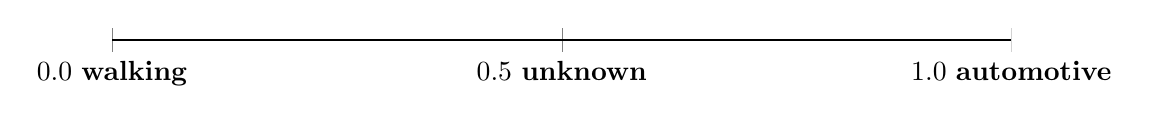
\begin{tikzpicture}
\begin{axis}[
    axis line style=thick,
    axis x line=middle,
    axis y line=none,
    width = 13cm,
    xtick distance=0.5,
    xticklabels={0, $0.0$ \textbf{walking}, $0.5$ \textbf{unknown}, $1.0$ \textbf{automotive}},
    major tick length = 0.3cm,
]
\end{axis}
\end{tikzpicture}
\note[itemize]{
\begin{itemize}
\item per rappresentare lo stato dell'utente i sensori utilizzano 
\item un valore reale compreso tra 0 e 1 detto confidenza 
\item quando minore di 0.5 indica lo stato walking, ossia che l'utente non si trova alla guida
\begin{itemize}
    \item dove 0 è la certezza massima
\end{itemize}
\item se uguale a 0.5 denota che il sensore non è in grado di determinare lo stato
\item quando maggiore di 0.5 indica lo stato automotive, ossia che l'utente sta guidando
\begin{itemize}
    \item dove 1 è la certezza massima
\end{itemize}
\end{itemize}
}
\end{frame}


\section{Il sensore Bluetooth}
\note[itemize]{
\item Il mio apporto al progetto GeneroCity è stato quello di realizzare il sensore Bluetooth per l'applicazione Android 
}

\begin{frame}{L'obbiettivo del sensore}
    \vspace{0.5cm}
    Rilevare connessioni Bluetooth con l'autoradio della macchina che l'utente sta guidando.
    \vspace{0.5cm}
    \begin{figure}
        \centering
        \includegraphics[width=0.5\linewidth]{assets/bt_logo.png}
    \end{figure}
\end{frame}
\note[itemize]{
\item si occupa di rilevare quando lo smartphone dell'utente si connette via Bluetooth ad un autoradio
\item assumendo con una certa probabilità che quando ciò accade l'utente si trova alla guida
\item per far ciò il sensore ha bisogno di ascoltare gli eventi di sistema riguardanti il Bluetooth
}

\begin{frame}{L'ascolto degli eventi di sistema}
\vspace{-0.5cm}
\begin{figure}
    \centering
    \includegraphics[width=0.9\linewidth]{assets/system_broadcast.png}
\end{figure}
\end{frame}
\note[itemize]{
\item difatti in Android le applicazioni possono registrarsi per essere notificate dal sistema operativo quando degli specifici eventi accadono
\item in questo caso al sensore interessano solamente gli eventi relativi al Bluetooth, più precisamente
\begin{itemize}
    \item la sua accensione e lo spegnimento
    \item la connessione o disconnessione di un dispositivo bluetooth
\end{itemize}
\item ogni volta che uno di questi eventi accade lo stato del sensore verrà aggiornato e la confidenza verrà coerentemente calcolata
}

\begin{frame}{Lo stato del sensore}
% \vspace{0.5cm}
\begin{columns}
    \begin{column}{0.5\textwidth}
        \begin{itemize}
            \item<2-> Stato del Bluetooth (acceso/spento)
            \item<3-> Lista dei dispositivi connessi
            \item<4-> Lista delle ultime 10 auto connesse
        \end{itemize}
    \end{column}
\end{columns}
\vspace{1cm}
\begin{columns}
    \begin{column}{0.1\linewidth}
    \end{column}
    \begin{column}{0.2\linewidth}
        \begin{figure}
            \centering
            \includegraphics<2->[width=0.6\linewidth]{assets/ic_bt_disabled.png}
        \end{figure}
    \end{column}
    \begin{column}{0.05\linewidth}
    \end{column}
    \begin{column}{0.2\linewidth}
        \begin{figure}
            \centering
            \includegraphics<3->[width=0.8\linewidth]{assets/ic_devices.png}
        \end{figure}
    \end{column}
    \begin{column}{0.05\linewidth}
    \end{column}
    \begin{column}{0.2\linewidth}
        \begin{figure}
            \centering
            \includegraphics<4->[width=0.7\linewidth]{assets/ic_car.png}
        \end{figure}
    \end{column}
    \begin{column}{0.1\linewidth}
    \end{column}
\end{columns}
\note[itemize]{
\begin{itemize}
\item in particolare lo stato del sensore è rappresentato da
    \begin{itemize}
        \item un flag che indica se il Bluetooth è acceso o spento
        \item la lista dei dispositivi che sono attualmente connessi
        \item la lista delle ultime 10 automobili che sono state connesse in precedenza
    \end{itemize}
\item questi dati saranno utilizzati per effettuare il calcolo della confidenza
\item a tale scopo è quindi importante rilevare e registrare le connessioni dello smartphone ad automobili
\end{itemize}
}
\end{frame}

\begin{frame}{Il rilevamento della connessione di un'automobile}
\begin{figure}
    \centering
    \includegraphics[width=\linewidth]{assets/algoritmo.png}
\end{figure}
\end{frame}
\note[itemize]{
\item infatti quando il sensore viene notificato di una nuova connessione sarà quindi eseguito il seguente algoritmo per rilevare le connessioni di automobili
\item nello specifico se il dispositivo connesso non è già presente nella lista delle auto
\item  viene verificato se la sua classe Bluetooth, ossia un codice che identifica la tipologia di dispositivo bluetooth, indica il tipo audiovideo car audio, classe che categorizza i dispositivi bluetooth relativi alle automobili
\item si è notato però che molto spesso essi utilizzano delle classi più generiche indicanti dei semplici dispositivi audiovideo
\item per questo motivo si è scelto di effettuare un controllo sul nome del dispositivo nel caso in cui la prima verifica fallisse
\item infatti il nome del bluetooth delle autoradio nella maggior parte dei casi corrisponde al nome del modello della relativa automobile oppure alla sua casa automobilistica
\item se il dispositivo viene identificato come una macchina allora verrà salvato nella lista dei dispositivi connessi con un attributo dal valore true che indica ciò
}

\section{Il calcolo della confidenza}
\note[itemize]{
\item come accennato precedentemente
\item ogni volta che lo stato del sensore cambia a seguito di un evento di sistema, come nel caso appena descritto, viene calcolata la confidenza in modo da aggiornare lo stato dell'utente di conseguenza
}

\begin{frame}{La confidenza restituita dal sensore Bluetooth}
\begin{itemize}
    \item<2-> Bluetooth spento $\to c=0.5$
    \item<3-> Nessun dispositivo connesso $\to c=0.0$
    \item<4-> Nessuna automobile tra i dispositivi connessi $\to c=0.1$
    \item<5-> Automobile connessa  $\to c\in[0.75, 1.0]$
\end{itemize}
\vspace{1.5cm}
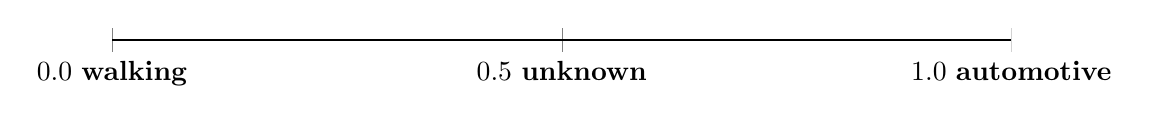
\begin{tikzpicture}
\begin{axis}[
    axis line style=thick,
    axis x line=middle,
    axis y line=none,
    width = 13cm,
    xtick distance=0.5,
    xticklabels={0, $0.0$ \textbf{walking}, $0.5$ \textbf{unknown}, $1.0$ \textbf{automotive}},
    major tick length = 0.3cm,
]
\end{axis}
\end{tikzpicture}
\note{
\begin{itemize}
    \item in particolare
    \item Se al momento del calcolo il Bluetooth è spento $\to c=0.5$ in quanto il sensore non può determinare lo stato dell'utente
    \item Se invece è acceso ma non c'è nessun dispositivo connesso $\to c=0.0$ sicuramente non connessa un macchina
    \item Altrimenti se ci sono dispositivi connessi ma nessuno di essi è un'auto $\to c=0.1$ dato che potrebbero essere presenti automobili non rilevate correttamente, viene quindi restituito lo stato walking ma con una probabilità leggermente più bassa
    \item Se invece un'automobile è connessa $\to c\in[0.75, 1.0]$ proporzionale al numero di connessioni
\end{itemize}
}
\end{frame}

\begin{frame}{L'incremento del numero di connessioni}
\begin{figure}
    \centering
    \includegraphics[width=\linewidth]{assets/algoritmo2.png}
\end{figure}
\end{frame}
\note[itemize]{
\item infatti quando viene rilevata una connessione di un'automobile con l'algoritmo precedentemente descritto
\item viene incrementato un attributo che si occupa di tenere traccia del numero di connessioni che quell'auto ha effettuato
\item ed infine viene salvato il dispositivo nella lista delle ultime automobili connesse, sovrascrivendo i vecchi dati se esso era già presente
}

\begin{frame}{Confidenza proporzionale al numero di connessioni}
\begin{columns}
    \begin{column}{0.3\textwidth}
        \begin{figure}
            \centering
            \includegraphics[width=\linewidth]{assets/car-bluetooth.png}
        \end{figure}
    \end{column}
    \begin{column}{0.6\textwidth}
        \begin{itemize}
            \item<1-> Il sensore deve riconoscere quando l'utente sta guidando e non sia un passeggero
            \item<2-> Si basa sul numero di connessioni effettuate con la stessa auto
            \item<3-> Più è un'auto usata frequentemente più è probabile che l'utente sia alla guida
            \item<4-> Restituire un valore proporzionale al numero di connessioni
        \end{itemize}
    \end{column}
\end{columns}
\note[itemize]{
\begin{itemize}
    \item questo perché
    \item importante sensore sia in grado di riconoscere quando l’utente si trova effettivamente alla guida e non sia un passeggero
    \item per discernere questi due casi esso si basa sul numero di connessioni effettuate verso la stessa autoradio
    \item assumendo che, se un'auto è molto utilizzata dall'utente, è altamente probabile che quando lo smartphone è connesso ad essa l'utente stia guidando
    \item dato che è verosimilmente una sua macchina
    \item e quindi, nel caso in cui un auto è connessa, il sensore restituirà una confidenza proporzionale al numero di connessioni che essa ha effettuato
\end{itemize}
}
\end{frame}

\begin{frame}{L'incremento esponenziale della confidenza}
\vspace{0.5cm}
\begin{tikzpicture}
\begin{axis}[
    axis lines = left,
    width = 13cm,
    height = 6cm,
    xmax=15,
    xlabel=Numero di connessioni,
    xtick={0,...,16},
    ymax=1,
    ylabel=Confidenza,
    ymajorgrids=true
]
  \addplot[
        maincolor,
        ultra thick,
        domain= 1:15,
        samples=100
    ] {0.75 + 0.0025 * (1.4^(x-1) -1)};
\end{axis}
\end{tikzpicture}
\end{frame}
\note[itemize]{
\item Per implementare questo aspetto si è deciso di utilizzare una funzione esponenziale
\item questo perché, a differenza di un approccio lineare, viene dato meno peso alle prime connessioni in quanto è più probabile che in questi casi l'utente sia un passeggero
\item inoltre l'incremento sarà progressivamente più elevato all'aumentare delle connessioni
\item nello specifico 
\begin{itemize}
    \item alla prima connessione viene restituito 0.75
    \item ed il valore rimarrà sotto lo 0.8 fino alla decima connessione
    \item per poi aumentare più velocemente fino alla quindicesima connessione per cui verrà restituito 1
    \item così come per tutte le connessioni successive ad essa
\end{itemize}
   
}

\begin{frame}[containsverbatim]{L'invio dei dati al server}
\vspace{0.25cm}
\begin{figure}
    \centering
    \includegraphics[width=0.8\linewidth]{assets/endpoint.png}
\end{figure}
% \vspace{-0.25cm}
\begin{columns}
\begin{column}{0.6\textwidth}
\begin{block}{Esempio di body inviato dal sensore}
\begin{Verbatim}[fontsize=\tiny]
{
   "action":"automotive",
   "confidence":0.75436,
   "data":{
      "bluetooth_enabled":true,
      "connected":[
         {
            "alias":"My Car",
            "bluetooth_class":"Handsfree",
            "connection_count":4,
            "device_name":"Fiat Punto",
            "is_car":true
         }
      ]
   },
   "datetime":"2024-10-21T15:43:24.525+02:00"
}
\end{Verbatim}
\end{block}
\end{column}
\end{columns}
\end{frame}
\note[itemize]{
\item come ogni sensore quando il suo stato cambia e la confidenza viene ricalcolata
\item il sensore Bluetooth invia una richiesta HTTP ad un apposito endpoint esposto dal backend di GeneroCity
\item che si occupa di memorizzare le rilevazioni effettuate dai sensori su un database
\item nel body richiesta si serializzano ...
\item questi dati vengono raccolti per allenare un modello di machine learning 
\begin{itemize}
    \item attualmente in sviluppo
    \item che sarà integrato integrato nell'applicazione
    \item con lo scopo di determinare l'effettivo stato dell'utente basandosi sulla confidenza calcolata da ogni sensore
    \item così da poter rilevare quando l'utente sta cercando un parcheggio senza la necessità di un suo input
\end{itemize}
}

% Se sono corto con i tempi aggiungere slide sul testing

\backmatter
\note[itemize]{
\item \textbf{Possibili domande}:
\item Testing:
    \begin{itemize}
        \item circa una 50 di test
        \item accendendo la macchina e connettendola al telefono
        \item verificando con un interfaccia grafica da me realizzata che veniva rilevata correttamente la connessione di una macchina
        \item e che la confidenza restituita fosse coerente con il numero di connessioni
    \end{itemize}
}
\end{document}
